\documentclass[11pt]{article}
\usepackage[utf8x]{inputenc}
\usepackage[english]{babel}
\usepackage{graphicx}
\usepackage{wrapfig}
\usepackage[margin=2cm, tmargin=2cm]{geometry}
\usepackage{color}
\usepackage{hyperref}
\usepackage{paralist}
\usepackage{wrapfig}
\usepackage{multicol}
\usepackage[normalem]{ulem}

\begin{document}
\noindent First name: \hfill {\scshape cyber} 2, {\scshape ensibs} Vannes, 2015-09-21 \\
Last name:
\begin{center}
	{\LARGE{Network evaluation}} \\ \vspace{10pt}
	\textbf{One handwritten} A4 sheet double sided allowed but no communication at all (unless you want your exam to be ended)!
	\textbf{Short} and right answers are the best (French or English). \underline{No need to debate, nor philosophize}. Final marking scheme may vary. \\
	Good luck!
\end{center}

\section{Design it (10 pts)}
	In this question you need to design several subnetworks. Starting from 172.17.0.0, give for each single subnetwork (no schema expected, though it can be helpful for you):
	\begin{itemize}
		\item the subnet mask and maximum number of hosts,
		\item the network IP address,
		\item the first node IP address,
		\item the last node IP address,
		\item the broadcast IP address.
		%\item the CIDR of the "super-network".
	\end{itemize}
	Sub-networks to be designed are:
	\begin{enumerate}
		\item 1000 machines for the students,
		\item 30 machines for the network services (DNS server, web, NAS...),
		\item 40 machines for the network lab,
		\item 500 machines for the teachers and workers,
		\item 14 machines for experimental purposes.
	\end{enumerate}
Use Table \ref{tab:design} on the fourth page.

\section{OSI model (2 pts)}
	Give the name and a short overview of the four first layers:
\pagebreak

\section{Routing decision (2 pts)}
	\subsection{Definitions}
		What are the definitions of: \emph{router}, \emph{routing algorithm} and \emph{forwarding}? (You can make up these three definitions in one sentence).
\vspace{3cm}

	\subsection{Next NIC?}
		\begin{table}[h]
		  \centering
		      \begin{tabular}{llll}
		      		\verb+Route #+	&	\verb+Destination+	& \verb+Genmask+		& \verb+Iface+ \\
		      		R0				&	\verb+0.0.0.0+ 		& \verb+/0+		 		& \verb+s0+ \\
		      		R1				&	\verb+10.0.0.0+		& \verb+/8+				& \verb+eth0+ \\
		      		R2				&	\verb+212.27.60.0+	& \verb+/22+			& \verb+s1+ \\
		      		R3				&	\verb+80.10.200.0+	& \verb+/22+			& \verb+s2+ \\
		      		R4				&	\verb+192.168.0.0+	& \verb+255.255.255.0+	& \verb+eth1+ \\
		      		R5				&	\verb+192.168.3.0+	& \verb+255.255.255.0+	& \verb+eth0+ \\
		      		R6				&	\verb+192.168.5.0+	& \verb+255.255.255.128+& \verb+eth1+ \\
		      \end{tabular}
		      \caption{Routing table}
		  \label{tab:routing}
		\end{table}

		According to the routing Table \ref{tab:routing}:
		\begin{itemize}
			\item What are the (optional) missing details ?
			\item Where will be forwarded packet with destinations:
			\begin{itemize}
				\item 198.41.191.47?
				\item 192.168.4.3?
				\item 192.168.1.1?
				\item 80.10.201.0?
				\item 80.10.210.0?
				\item 10.128.0.4?
				\item 212.27.61.1?
			\end{itemize}
			\item Is there routes than can be summarized ? If yes, which one(s) into which "super-network"?
		\end{itemize}

\pagebreak
\section{What layer is it ? (2 pts)}
	Complete the table \ref{tab:protocol} with (include the default port, if any, in brackets -see HTTP example-): \sout{HTTP}, HTTPS, TCP, UDP, MAC, IP, telnet, ssh, ftp, IEEE 802.11, IEEE 802.15.2, DNS, SIP, TLS, ICMP, IS-IS, RIP.
	\subsection{Next NIC?}
		\renewcommand{\arraystretch}{1.5}
			\begin{table}[h]
			%  \centering
			      \begin{tabular}{l|l}
			      		\verb+Layer+	&	\verb+Protocols+	\\ \hline
						\verb+*+		&	\\
			      		7				&	HTTP(80),			\\
			      		6				&	\\
			      		5				&	\\
			      		4				&	\\
			      		3				&	\\
			      		2				&	\\
			      		1				&	\\
			      \end{tabular}
			      \caption{Protocol table}
			  \label{tab:protocol}
			\end{table}
		\renewcommand{\arraystretch}{1.0}

	\section{Who is it? (2 pts)}
		What can you conclude according to the two packets shown in \ref{fig:dns}?
		\begin{figure}[h]
			\begin{center}
				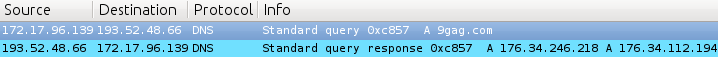
\includegraphics[width=18cm]{dns.png}
				\caption{Two lonely packets}
				\label{fig:dns}
			\end{center}
		\end{figure}
		\vspace{1cm}

\section{Bonus question (0.5 pts)}
	\subsection{DEF CON 22 Hacking Conference}
		What did you learn by watching to the video named \emph{Blinding The Surveillance State By Christopher Soghoian}?
\pagebreak

You may want not to write the whole IP addresses but only the changing bytes.
\renewcommand{\arraystretch}{1.5}
\setlength{\tabcolsep}{14pt}
	\begin{table}[h]
	  \centering
		  \begin{tabular}{|l|l|l|l|l|l|l|}
			  \hline
				Network ID	&	Mask (CIDR)	& \# hosts	& Network	&	First node	&	Last node	&	Broadcast	\\ \hline
				&&&&&&	\\ \hline
				&&&&&&	\\ \hline
				&&&&&&	\\ \hline
				&&&&&&	\\ \hline
				&&&&&&	\\ \hline
				&&&&&&	\\ \hline
				&&&&&&	\\ \hline
				&&&&&&	\\ \hline
				&&&&&&	\\ \hline
				&&&&&&	\\ \hline
				&&&&&&	\\ \hline
		  \end{tabular}
		  \caption{Designed networks}
	  \label{tab:design}
	\end{table}
\renewcommand{\arraystretch}{1.0}
\end{document}
